\documentclass[12pt,a4paper]{article}

% ── Packages ─────────────────────────────────────────────────────────────────
\usepackage[a4paper,top=2.5cm,bottom=2.5cm,left=2.5cm,right=2.5cm,headheight=14pt]{geometry}
\usepackage[T1]{fontenc}
\usepackage[utf8]{inputenc}
\usepackage{setspace}
\usepackage{parskip}
\usepackage{titlesec}
\usepackage{booktabs}
\usepackage{longtable}
\usepackage{array}
\usepackage{xcolor}
\usepackage{graphicx}
\usepackage{hyperref}
\usepackage{enumitem}
\usepackage{fancyhdr}
\usepackage{lastpage}
\usepackage{tcolorbox}
\usepackage{amsmath}
\usepackage{amssymb}
\usepackage{listings}
\usepackage{caption}
\usepackage{tikz}
\usepackage{pgf}
\usetikzlibrary{shapes.geometric,shapes.multipart,arrows.meta,positioning,
                fit,backgrounds,calc,decorations.pathreplacing,shadows}

% ── Colours ──────────────────────────────────────────────────────────────────
\definecolor{ksiugold}{RGB}{180,140,0}
\definecolor{ksiudark}{RGB}{30,30,30}
\definecolor{lightgray}{RGB}{245,245,245}
\definecolor{codegreen}{RGB}{0,128,0}
\definecolor{codegray}{RGB}{128,128,128}
\definecolor{codered}{RGB}{180,0,0}
\definecolor{stageblue}{RGB}{52,101,164}
\definecolor{stageorange}{RGB}{206,92,0}
\definecolor{stagegreen}{RGB}{78,153,56}
\definecolor{stagered}{RGB}{164,0,0}
\definecolor{stagegray}{RGB}{85,87,83}
\definecolor{pkcolor}{RGB}{180,60,0}
\definecolor{fkcolor}{RGB}{0,80,160}
\definecolor{tableheader}{RGB}{52,101,164}

% ── Hyperref ─────────────────────────────────────────────────────────────────
\hypersetup{colorlinks=true,linkcolor=ksiugold,urlcolor=ksiugold,
            citecolor=ksiugold,pdftitle={ACR-QA Assignment 3},
            pdfauthor={Ahmed Mahmoud Abbas}}

% ── Headers/footers ──────────────────────────────────────────────────────────
\pagestyle{fancy}\fancyhf{}
\fancyhead[L]{\small Ahmed Mahmoud Abbas}
\fancyhead[R]{\small ACR-QA --- Assignment 3}
\fancyfoot[C]{\small Page \thepage\ of \pageref{LastPage}}
\renewcommand{\headrulewidth}{0.4pt}

% ── Section formatting ───────────────────────────────────────────────────────
\titleformat{\section}{\large\bfseries\color{ksiugold}}{\thesection.}{0.6em}{}[\titlerule]
\titleformat{\subsection}{\normalsize\bfseries\color{ksiudark}}{\thesubsection.}{0.5em}{}
\titleformat{\subsubsection}{\normalsize\itshape\color{ksiudark}}{\thesubsubsection.}{0.5em}{}

% ── Code listing style ───────────────────────────────────────────────────────
\lstset{basicstyle=\ttfamily\small,keywordstyle=\color{codered}\bfseries,
  commentstyle=\color{codegreen},numberstyle=\tiny\color{codegray},
  numbers=left,stepnumber=1,frame=single,backgroundcolor=\color{lightgray},
  breaklines=true,showstringspaces=false,captionpos=b}

% ── Line spacing ─────────────────────────────────────────────────────────────
\setstretch{1.15}

% ── TikZ styles ──────────────────────────────────────────────────────────────
\tikzset{
  pipenode/.style={rectangle,rounded corners=4pt,draw=#1!70!black,
    fill=#1!15,text width=2.4cm,minimum height=0.9cm,align=center,
    font=\small\bfseries,drop shadow},
  pipearrow/.style={-Stealth,thick,color=ksiudark},
  fanout/.style={rectangle,rounded corners=3pt,draw=stagegreen!70!black,
    fill=stagegreen!12,text width=2.2cm,minimum height=0.7cm,align=center,
    font=\footnotesize},
  erbox/.style={rectangle,draw=tableheader!80!black,fill=tableheader!10,
    text width=3.6cm,align=left,font=\footnotesize,drop shadow},
  erhead/.style={rectangle,draw=tableheader!80!black,fill=tableheader,
    text width=3.6cm,align=center,font=\footnotesize\bfseries\color{white}},
  errel/.style={-Stealth,thick,color=stageblue!70!black},
  erlabel/.style={font=\scriptsize\itshape,color=stagegray},
}

% ═══════════════════════════════════════════════════════════════════════════
\begin{document}
% ═══════════════════════════════════════════════════════════════════════════

%% ── Title page ──────────────────────────────────────────────────────────────
\begin{titlepage}
\centering\vspace*{1cm}
{\Large\bfseries Faculty of Computer Science and Engineering\\[0.3em]
Computer Science / Software Engineering Programme\\[0.3em]
CSE494 \& AIE494 --- Graduation Project 2}
\vspace{1.5cm}

{\Huge\bfseries\color{ksiugold} Assignment 03}
\vspace{0.8cm}

{\large\bfseries\color{codered} Submission deadline: 9 April 2026}
\vspace{1.5cm}

\begin{tabular}{ll}
\textbf{Student Name:} & Ahmed Mahmoud Abbas \\[0.3em]
\textbf{Student ID:}   & 222101213 \\[0.3em]
\textbf{Supervisor:}   & Dr.\ Samy AbdelNabi \\[0.3em]
\textbf{Programme:}    & Computer Science \\[0.3em]
\textbf{Academic Year:}& 2025--2026 \\[0.3em]
\textbf{Date:}         & 17 March 2026 \\
\end{tabular}
\vspace{1.5cm}

{\large\bfseries Project Title:}\\[0.4em]
{\Large ACR-QA: Automated Code Review \& Quality Assurance Platform}\\[0.3em]
{\normalsize Language-Agnostic with RAG-Enhanced AI Explanations --- v2.8.0}
\vspace{2cm}

{\footnotesize King Salman International University --- El Tor Campus --- South Sinai\\
\texttt{www.ksiu.edu.eg}}
\end{titlepage}

\newpage
\tableofcontents
\newpage

% ═══════════════════════════════════════════════════════════════════════════
\section{Summary}
% ═══════════════════════════════════════════════════════════════════════════

This assignment serves three purposes.  First, it allows me to assess my own progress
against the targets set in Assignments 1 and 2 and the original project proposal.
Second, it requires me to plan the final project report before writing it, by producing a
structured outline and a detailed draft of the ``Doing'' section.  Third, it provides an
opportunity to receive formative feedback from my supervisor, Dr.\ Samy AbdelNabi,
before the final report submission in June 2026.

\textbf{Question 1} presents a complete outline of the final project report including
sections, subsections, appendices, and estimated word counts.  \textbf{Question 2}
is a full draft of the ``Do'' part, covering literature search and resource evaluation
(Part a), methodological approach and justification (Part b), activities and decisions
made during execution (Part c), and observations on structure and style (Part d).

% ═══════════════════════════════════════════════════════════════════════════
\section{Question 1: Report Outline (20 marks)}
% ═══════════════════════════════════════════════════════════════════════════

\subsection{Outline Plan}

The final report targets approximately \textbf{6,000 words} within the required
5,000--7,000 range.  The structure follows the \emph{plan--do--review--communicate}
framework from the project report guide.

\begin{longtable}{p{0.45\linewidth}p{0.13\linewidth}p{0.36\linewidth}}
\toprule
\textbf{Section / Subsection} & \textbf{Est.\ Words} & \textbf{Contents Summary}\\
\midrule\endfirsthead
\multicolumn{3}{c}{\small\itshape(Continued)}\\
\toprule\textbf{Section / Subsection}&\textbf{Est.\ Words}&\textbf{Contents Summary}\\
\midrule\endhead
\bottomrule
\endlastfoot

\textbf{1. Introduction} & 400
  & Problem statement, motivation, overview of deliverables, report road-map.\\
\quad 1.1 Background \& Motivation & 150
  & The cost of manual code review; gaps in existing automated tools; hallucination risk in AI explanations.\\
\quad 1.2 Project Aims \& Scope & 150
  & The five original aims; explicit in-scope and out-of-scope boundaries.\\
\quad 1.3 Report Structure & 100
  & One-sentence description of each remaining section.\\
\midrule

\textbf{2. Planning} & 500
  & How the project was designed before implementation.\\
\quad 2.1 Requirements Specification & 200
  & Functional and non-functional requirements; Volere 95\% compliance; acceptance criteria per phase.\\
\quad 2.2 Literature Search Strategy & 150
  & Three retrieval methods; search terms; initial source evaluation using PROVEN.\\
\quad 2.3 Risk Management & 150
  & Five identified risks with probability, impact, and mitigation strategies; contingency plans.\\
\midrule

\textbf{3. Doing} & 3,200
  & Core implementation narrative: what was built, how, and why.\\
\quad 3.1 System Architecture & 400
  & Updated v2.8 pipeline (7 stages + fan-out output); component interactions; design rationale.\\
\quad 3.2 Detection Layer & 350
  & Seven tools (Ruff, Semgrep, Bandit, Vulture, Radon, Secrets Detector, SCA Scanner); justification for each; parallel execution.\\
\quad 3.3 Normalisation \& Canonical Schema & 300
  & Universal finding format; 127 rule mappings; Pydantic v2 validation; cross-tool deduplication.\\
\quad 3.4 AI Explanation Engine (RAG) & 400
  & Rule retrieval; evidence-grounded prompting; Cerebras Llama 3.1 8B; entropy scoring; self-evaluation; fallback.\\
\quad 3.5 Policy-as-Code Engine & 250
  & \texttt{.acrqa.yml} schema; quality gate; severity overrides; CI/CD blocking; 9-repo calibration.\\
\quad 3.6 Test Gap Analyser & 200
  & AST-based untested function detection; cyclomatic complexity ranking; competitive differentiation.\\
\quad 3.7 Testing \& Calibration & 300
  & 297-test suite; sub-6\,s runtime; 9-repo calibration study; threshold tuning decisions.\\
\quad 3.8 Evaluation Results & 1,000
  & Precision/recall/F1 per repository; DVPWA ground-truth recall (50\%); OWASP 9/10 coverage; comparative benchmark vs.\ raw tools; user study design.\\
\midrule

\textbf{4. Review} & 900
  & Critical reflection on results, decisions made, and limitations.\\
\quad 4.1 Achievement Against Aims & 300
  & Mapping each of the five original aims to concrete evidence of delivery.\\
\quad 4.2 Limitations & 300
  & DVPWA recall gaps (CSRF, IDOR, debug mode); Python-only language scope; user study pending.\\
\quad 4.3 Lessons Learnt & 150
  & API integration complexity; importance of empirical calibration; scope discipline.\\
\quad 4.4 Future Work & 150
  & JavaScript/TypeScript adapter; cloud deployment; expanded user study (n\,=\,10).\\
\midrule

\textbf{5. Conclusion} & 300
  & Summary of contributions; significance for academic and industry contexts; graduation readiness.\\
\midrule

\textbf{References} & 200 & Harvard-style (9 sources).\\
\midrule

\textbf{Appendix A: Database Schema SQL}    & ---
  & Full DDL for all five PostgreSQL tables with constraints and indexes.\\
\textbf{Appendix B: Canonical Finding JSON} & ---
  & Sample normalised finding (SQL injection) with all fields annotated.\\
\textbf{Appendix C: \texttt{.acrqa.yml} Template} & ---
  & Fully documented policy configuration file.\\
\textbf{Appendix D: OWASP Coverage Table}  & ---
  & All 10 OWASP Top 10 categories with ACR-QA rule IDs and CWEs.\\
\textbf{Appendix E: Pipeline Architecture Diagram} & ---
  & v2.8 system diagram with all stages and output fan-out (TikZ).\\
\textbf{Appendix F: ER Diagram}            & ---
  & Entity-Relationship diagram for the five-table provenance schema (TikZ).\\
\textbf{Appendix G: User Study Materials}  & ---
  & Group A / Group B survey instruments; results template; analysis script.\\
\bottomrule
\end{longtable}

\vspace{0.5em}
\noindent\textbf{Total body word count target:} $\approx$\,\textbf{6,000 words}.
Appendices are not counted towards the word limit.

\subsubsection*{Narrative visible from section titles alone}
Introduction $\to$ Planning (why this approach) $\to$ Doing (building and evaluating)
$\to$ Review (reflecting honestly on results) $\to$ Conclusion.

% ═══════════════════════════════════════════════════════════════════════════
\section{Question 2: Draft of the ``Do'' Part (80 marks)}
% ═══════════════════════════════════════════════════════════════════════════

\noindent\textit{Word count of this draft (Sections a--c): approximately
\textbf{3,200 words}, consistent with the 3,200-word allocation planned for
Section 3 (Doing) in the report outline above.}

\bigskip

\noindent\textbf{Introduction to the Doing Section}

ACR-QA v2.8 is a fully automated, AI-powered code review and quality assurance
platform built over eight months (October 2025 -- March 2026).  Starting from a
Python adapter prototype in October 2025, the project evolved through two phases
into an enterprise-ready product with seven integrated static analysis tools, a
RAG-enhanced explanation engine, a Policy-as-Code quality gate, a Test Gap
Analyser, and a 297-test continuous integration suite.  This section describes what
was built, how each decision was made, and what evidence will support each claim in
the final report.

% ─────────────────────────────────────────────────────────────────────────────
\subsection{(a) Literature Search and Resources Identified (12 marks)}
% ─────────────────────────────────────────────────────────────────────────────

\subsubsection{Knowledge Gaps Identified at Project Start}

At the start of the project in October 2025, four areas were identified where my
existing knowledge was insufficient:

\begin{enumerate}[leftmargin=1.5em]
  \item \textbf{Retrieval-Augmented Generation (RAG).}  I understood LLM theory
  from coursework but had not implemented a RAG pipeline.  I needed to understand
  hallucination measurement, vector retrieval, and evidence-grounded prompting
  before building the explanation engine.

  \item \textbf{Multi-tool static analysis normalisation.}  I was familiar with
  individual linters (Ruff, Bandit) but had not unified outputs from seven tools
  with incompatible JSON schemas into a single canonical format.

  \item \textbf{Developer adoption barriers for static analysis.}  I needed
  empirical evidence for \emph{why} developers ignore automated tools so that design
  decisions --- severity prioritisation, actionable AI explanations, feedback loop
  --- could be academically justified rather than assumed.

  \item \textbf{OWASP Top 10 and CWE mapping.}  I needed to understand how to map
  low-level rule IDs to OWASP categories and CWE identifiers to make the compliance
  reporting feature credible and academically grounded.
\end{enumerate}

\subsubsection{Search Methods, Resources, and Their Usefulness}

Three distinct retrieval methods were used throughout the project log (October
2025 -- March 2026).

\textbf{Method 1 --- Academic database search (IEEE Xplore, ACM Digital Library,
Google Scholar).}  Targeted keyword queries included \emph{``retrieval augmented
generation hallucination reduction''}, \emph{``multi-language static code analysis
adapter pattern''}, and \emph{``developer static analysis tool adoption barriers''}.
This produced four peer-reviewed sources with direct relevance.  Searches took
30--60 minutes per query but consistently returned high-quality, citable material.
\emph{Successes:} found Johnson et al.\ (2013) and Lewis et al.\ (2020) on the first
query attempt each.  \emph{Failures:} two AI-suggested paper titles (found via Method
3) did not exist in IEEE Xplore; both were discarded immediately after verification.

\textbf{Method 2 --- Official tool documentation (Semgrep, Ruff, Bandit, Cerebras
API, GitHub REST API).}  Consulted directly for implementation details: output JSON
schemas, API authentication flows, rule syntax, and rate-limit behaviour.  Highly
authoritative and directly applicable, though narrow in scope.  Key outcome: the
Semgrep documentation revealed the YAML rule authoring syntax, which enabled five
new custom detection patterns (XSS via \texttt{render\_template\_string}, SSRF, JWT
\texttt{none} algorithm bypass, lxml XXE, open redirect) added in v2.8 to close gaps
identified during the four-repository benchmark.

\textbf{Method 3 --- AI-assisted synthesis (Claude, ChatGPT).}  Used conversationally
to synthesise trends across papers, locate non-indexed whitepapers, and quickly
identify suitable deliberately vulnerable repositories (DVPWA, Pygoat, VulPy, DSVW)
for use as evaluation targets.  Fast (5--10 minutes per query) but required
independent verification of every suggested source before inclusion.

\subsubsection{Source Quality Evaluation Using PROVEN}

The PROVEN framework (Provenance, Relevance, Ownership, Verification, Evidence,
Nature) from Assignment 2 was applied consistently to four key sources.

\medskip
\noindent\textbf{Source 1 --- Johnson et al.\ (2013), ``Why Don't Software
Developers Use Static Analysis Tools to Find Bugs?''}

\begin{itemize}[leftmargin=1.5em,itemsep=2pt]
  \item \textbf{Provenance:} IEEE Transactions on Software Engineering ---
  highest-tier peer-reviewed venue; double-blind review.
  \item \textbf{Relevance:} Identifies three adoption barriers (false positive
  noise, lack of actionable guidance, workflow friction) that directly shaped
  ACR-QA's severity prioritisation, RAG explanations, and the developer
  feedback loop.
  \item \textbf{Ownership:} Microsoft Research + University of Washington;
  no commercial conflict.
  \item \textbf{Verification:} 2,847+ citations; qualitative methodology
  openly reproducible.
  \item \textbf{Evidence:} Empirical user study with 20 professional developers;
  grounded theory coding.
  \item \textbf{Nature:} Rigorous academic research.
  \item \textbf{Assessment:} Excellent.  Primary justification for the feedback
  loop, severity ordering, and AI explanation design.
\end{itemize}

\medskip
\noindent\textbf{Source 2 --- Lewis et al.\ (2020), ``Retrieval-Augmented
Generation for Knowledge-Intensive NLP Tasks'' (NeurIPS)}

\begin{itemize}[leftmargin=1.5em,itemsep=2pt]
  \item \textbf{Provenance:} NeurIPS 2020 --- top-tier ML conference.
  \item \textbf{Relevance:} Foundational RAG paper; directly informs the ACR-QA
  explanation engine design: retrieve rule definition, ground prompt, generate.
  \item \textbf{Ownership:} Facebook AI Research; no conflict.
  \item \textbf{Verification:} 10,000+ citations; model weights publicly available.
  \item \textbf{Evidence:} Empirical benchmarks across knowledge-intensive NLP tasks.
  \item \textbf{Nature:} Rigorous academic research with strong reproducibility.
  \item \textbf{Assessment:} Excellent.  Provides theoretical grounding for choosing
  RAG over direct LLM prompting.
\end{itemize}

\medskip
\noindent\textbf{Source 3 --- CustomGPT (2025), ``RAG API vs Traditional LLM APIs''}

\begin{itemize}[leftmargin=1.5em,itemsep=2pt]
  \item \textbf{Provenance:} Industry whitepaper; not peer-reviewed.
  \item \textbf{Relevance:} Quantitative hallucination reduction claims
  (42--68\%) for RAG vs.\ direct API calls; supports architecture decision.
  \item \textbf{Ownership:} CustomGPT engineering team --- commercial interest
  in RAG products.
  \item \textbf{Verification:} Methodology described but evaluation dataset
  not publicly available.
  \item \textbf{Evidence:} 500 technical Q\&A pairs; GPT-4 baseline comparison.
  \item \textbf{Nature:} Applied industry research.
  \item \textbf{Assessment:} Good as supporting evidence only; supplemented
  with Lewis et al.\ (2020) for academic rigour.
\end{itemize}

\medskip
\noindent\textbf{Source 4 --- IEEE (2023), ``Towards Multi-Language Static Code
Analysis'' (ISSREW)}

\begin{itemize}[leftmargin=1.5em,itemsep=2pt]
  \item \textbf{Provenance:} IEEE ISSREW 2023 --- peer-reviewed workshop.
  \item \textbf{Relevance:} Validates the adapter pattern for multi-language
  analysis; empirical overhead of 2--8\% for normalisation, consistent with
  ACR-QA's measured $<500$\,ms.
  \item \textbf{Ownership:} University researchers; no conflict.
  \item \textbf{Verification:} DOI-registered; reproducible benchmarks published.
  \item \textbf{Evidence:} Performance data across four language adapters.
  \item \textbf{Nature:} Academic research.
  \item \textbf{Assessment:} Excellent.  Justifies canonical schema architecture
  and confirms normalisation feasibility within time budget.
\end{itemize}

\subsubsection{Steps to Improve Future Literature Searching}

Three practical improvements emerged from reviewing the project log:

\begin{enumerate}[leftmargin=1.5em]
  \item \textbf{Verify AI-suggested sources immediately.}  Two paper titles
  suggested by AI assistants did not exist; future searches will cross-reference
  every suggested title in IEEE Xplore before recording it in the log.
  \item \textbf{Search for labelled evaluation datasets earlier.}  Locating
  ground-truth vulnerability datasets (beyond DVPWA) later in the project
  limited recall measurement to one repository.  Earlier discovery would enable
  rigorous recall measurement across all four.
  \item \textbf{Use structured keyword matrices.}  A systematic
  (concept)$\times$(method)$\times$(year range) matrix would ensure coverage
  across sub-fields rather than ad hoc queries.
\end{enumerate}

% ─────────────────────────────────────────────────────────────────────────────
\subsection{(b) Your Approach (24 marks)}
% ─────────────────────────────────────────────────────────────────────────────

\subsubsection{Approach and Methods}

ACR-QA was built using a \textbf{modular, pipeline-based architecture} that combines
multi-tool static analysis with a RAG-enhanced AI explanation engine.  The actual
v2.8 pipeline, as implemented in \texttt{CORE/main.py}, differs from the v2.5
architecture document in three important ways --- an important distinction documented
here as the assignment requires describing the work as it was actually done:

\begin{quote}
\footnotesize
\texttt{[0] Rate Limit Check $\to$ [1] Create DB Run $\to$ [2] Detection (7 tools, parallel) $\to$}\\
\texttt{[2b] Extra Scanners (Secrets + SCA) $\to$ [3] Normalise / Filter / Dedup / Cap / Sort $\to$}\\
\texttt{[4] AI Explanation (RAG) $\to$ [5] Quality Gate $\to$ [6] Output Fan-out}
\end{quote}

The three changes from v2.5: (i) a \textbf{rate limit check} was added at step
[0] after Redis integration; (ii) \textbf{Secrets Detection and SCA Scanning} run
as a separate sequential stage [2b] after the six parallel tools because they
require different inputs; and (iii) the \textbf{Quality Gate moved to after} AI
Explanation --- the old architecture document incorrectly placed it before
explanation, which would gate on un-enriched findings.

Figure~\ref{fig:pipeline} (Appendix~\ref{app:pipeline}) shows the corrected
v2.8 pipeline.

The technical stack is: Python 3.11 (CORE pipeline), Flask (REST API + dashboard),
PostgreSQL 15 (five-table provenance schema), Redis (rate limiting and explanation
caching), Prometheus + Grafana (observability), GitHub Actions (CI/CD), and Docker
Compose (5-service deployment).

The AI explanation engine uses RAG: for each finding, the system performs a
deterministic dictionary lookup of the matching rule in \texttt{config/rules.yml}
(66 rules with rationale, remediation steps, and code examples), constructs an
evidence-grounded prompt including the 3-line code context, calls Cerebras
Llama 3.1 8B, then measures response consistency across three temperature variants
(Semantic Entropy scoring, 0--1 range) and runs a self-evaluation step where the
model rates its own output on relevance, accuracy, and clarity (1--5 scale).

\subsubsection{Justification for This Approach vs.\ Alternatives}

Table~\ref{tab:approaches} compares the chosen approach against two credible
alternatives.

\begin{table}[ht]
\centering
\caption{Architectural approach comparison}
\label{tab:approaches}
\small
\begin{tabular}{p{0.18\linewidth}p{0.26\linewidth}p{0.26\linewidth}p{0.24\linewidth}}
\toprule
\textbf{Criterion} &
\textbf{ACR-QA (chosen):\newline Multi-tool + RAG} &
\textbf{Alt.\ A:\newline Single tool + direct LLM} &
\textbf{Alt.\ B:\newline ML classifier from scratch} \\
\midrule
Detection breadth & High: 7 tools cover security, style, complexity, dead code, duplication
  & Low: one tool's rule set only
  & Medium: depends on training data \\
Hallucination control & Measurable entropy score + rule grounding
  & No grounding; hallucinations undetectable
  & N/A (not generative) \\
Cost & Zero recurring (free APIs)
  & Recurring LLM cost per call
  & High: GPU + labelled dataset \\
Timeline & High: composable, testable incrementally
  & High: simpler architecture
  & Low: multi-month training \\
Explainability & Evidence-grounded, cites rule ID
  & Opaque
  & Opaque \\
\midrule
Advantages & Breadth; measurable quality; zero cost
  & Simpler to build
  & Potentially higher recall \\
Disadvantages & Higher integration complexity
  & Hallucination risk; narrow scope
  & Infeasible in 8 months \\
\bottomrule
\end{tabular}
\end{table}

Alternative A was rejected because Johnson et al.\ (2013) show that a single tool
producing high false-positive noise causes developer abandonment; covering only one
detection category would miss the cross-cutting issues that matter most to teams.
Alternative B was rejected as infeasible within the 8-month timeline: acquiring
sufficient labelled vulnerability data and training a model would consume the entire
Phase 1 window.  The chosen approach trades integration complexity for breadth,
measurability, and zero running cost.

\subsubsection{Software and Modelling Tools Used, with Limitations}

\begin{itemize}[leftmargin=1.5em]
  \item \textbf{Ruff} (Python linter, Rust-based): style violations, unused imports,
  modernisation.  10--100$\times$ faster than Pylint/Flake8; replaces six legacy tools.
  \emph{Limitation:} Python-only.

  \item \textbf{Bandit} (Python security scanner): eval, exec, pickle, SQL injection,
  weak crypto, hardcoded secrets.  100\% security precision across all four evaluation
  repositories.  \emph{Limitation:} Python-specific; cannot detect CSRF or IDOR
  architecturally.

  \item \textbf{Semgrep} (pattern-based, multi-language): five custom YAML rules
  (XSS, SSRF, JWT bypass, XXE, open redirect) added in v2.8 to close benchmark gaps.
  \emph{Limitation:} rules must be written manually; zero findings on DVPWA until
  custom rules were authored.

  \item \textbf{Vulture} (dead code detector): 241 findings across four repos.
  \emph{Limitation:} $\approx$5\% false positives on Django template-called functions
  (cannot trace \texttt{urls.py} $\to$ \texttt{views.py} references).

  \item \textbf{Radon} (cyclomatic complexity): mathematical metric; zero false
  positives possible.  Flags functions with CC\,$>$\,10.  \emph{Limitation:} reports
  complexity, not root cause.

  \item \textbf{jscpd} (code duplication, token-based): zero false positives.
  \emph{Limitation:} sensitive to minimum block-size threshold; too small a threshold
  floods results with trivial matches.

  \item \textbf{Secrets Detector} (custom, \texttt{CORE/engines/secrets\_detector.py}):
  pattern-based secret and credential scanning.  \emph{Limitation:} regex-based; cannot
  detect secrets obfuscated as environment variable names.

  \item \textbf{SCA Scanner} (custom, \texttt{CORE/engines/sca\_scanner.py}):
  Software Composition Analysis for known-vulnerable dependencies.
  \emph{Limitation:} database currency depends on manual updates.

  \item \textbf{Cerebras Llama 3.1 8B (free tier)}: mean explanation latency 800\,ms.
  Chosen over GPT-4 (\$30/1M tokens) because Cerebras provides free-tier access.
  \emph{Limitation:} smaller model; requires RAG grounding for acceptable accuracy.

  \item \textbf{PostgreSQL 15 + Redis}: provenance database and caching layer.
  \emph{Limitation:} Redis is optional; system degrades gracefully to in-memory
  rate limiting when Redis is unavailable.

  \item \textbf{Docker Compose (5 services)}: App, PostgreSQL, Redis, Prometheus,
  Grafana.  Single-command deployment, no cloud required.  \emph{Limitation:} no
  horizontal scaling support; sufficient for single-instance academic deployment.

  \item \textbf{GitHub Actions}: CI/CD triggering 297 tests on every push; free for
  open-source repositories.  \emph{Limitation:} 2,000 free minutes/month ceiling
  (not approached during this project).
\end{itemize}

% ─────────────────────────────────────────────────────────────────────────────
\subsection{(c) Activities and Decisions Made (24 marks)}
% ─────────────────────────────────────────────────────────────────────────────

\subsubsection{Summary of Activities by Phase}

\textbf{Phase 1 --- Foundation (October 2025 -- January 2026).}
The Python adapter was implemented and validated in October 2025, ahead of schedule,
producing canonical JSON findings from six analysis tools.  The canonical schema was
designed with 47 initial rule IDs.  Docker Compose orchestration and the five-table
PostgreSQL schema were operational by November.  The RAG explanation engine ---
Cerebras API integration, entropy scoring, template fallback --- was completed in
December.  GitHub Actions CI/CD with the 297-test suite was green by January 2026,
completing Phase 1.

\textbf{Phase 2 --- Enterprise Features (January -- March 2026).}
Between January and March 2026, ACR-QA evolved from v2.0 (working prototype) to
v2.8.0 (enterprise release).  Six major additions were made:

\begin{itemize}[leftmargin=1.5em,itemsep=3pt]
  \item \textbf{Policy-as-Code engine (v2.3):} The \texttt{.acrqa.yml} configuration
  file enables teams to define rule suppression, severity overrides, path exclusions,
  minimum severity thresholds, quality gate thresholds, autofix policy, and AI
  explanation limits --- all version-controlled alongside the codebase.  A CLI
  validator (\texttt{validate\_config.py}) and template generator were added.

  \item \textbf{Test Gap Analyser (v2.4):} A novel feature using Python's
  \texttt{ast} module to identify untested functions ranked by cyclomatic complexity.
  Applied to the ACR-QA codebase itself: 103 functions scanned, 40 identified as
  untested, with the most complex prioritised.  No commercial competitor offers this
  feature.

  \item \textbf{OWASP Top 10 compliance mapping (v2.5):} Every security finding is
  tagged with an OWASP 2021 category and a CWE identifier.  Coverage: 9 of 10
  categories.  A09 (Logging Failures / CWE-778) remains unmapped --- no Bandit or
  Semgrep rule currently addresses Python logging failures.

  \item \textbf{Developer Fatigue Tuner and Feedback Tuner (v2.6):} The thumbs
  up/down feedback mechanism per finding feeds into
  \texttt{scripts/feedback\_tuner.py}, which auto-generates severity overrides to
  suppress future false-positive noise for that repository.

  \item \textbf{Four-repository benchmark evaluation (v2.7--v2.8):} Systematic
  evaluation against DVPWA, Pygoat, VulPy, and DSVW with per-tool precision
  analysis and calibrated quality gate defaults derived from a 9-repository study.

  \item \textbf{Five new Semgrep rules (v2.8):} \texttt{flask-xss-render-string}
  (CWE-79), \texttt{ssrf-requests-user-url} (CWE-918),
  \texttt{jwt-none-algorithm} (CWE-347), \texttt{lxml-xxe} (CWE-611), and
  \texttt{open-redirect} (CWE-601) --- authored to close detection gaps found during
  the benchmark.
\end{itemize}

\subsubsection{Key Decisions and Justifications}

\textbf{Decision 1: Expand scope from PR-diff-only to full repository analysis.}

Assignment 2 planned to analyse only pull-request diffs.  This was relaxed during
Phase 1: batch analysis of full repositories is needed for the evaluation benchmark
and the Test Gap Analyser requires whole-repository AST traversal.  PR-diff mode is
retained via the \texttt{--diff-only} CLI flag.  \emph{Justification:} full-repository
analysis makes results directly comparable to SonarQube and enables the evaluation
study required by the assignment.

\textbf{Decision 2: Replace pgvector with dictionary-backed rule lookup.}

Assignment 2 planned to use pgvector for semantic retrieval of rule definitions.
After prototyping, this was replaced with a deterministic dictionary lookup keyed on
canonical rule ID.  \emph{Justification:} the knowledge base is small (66 rules) and
every finding already carries an exact canonical rule ID --- semantic search adds
latency and infrastructure complexity without improving output quality.  This
eliminated a runtime dependency and reduced mean explanation latency from an estimated
1,400\,ms (with vector retrieval overhead) to 800\,ms (direct lookup + LLM call).

\textbf{Decision 3: Calibrate quality gate defaults from a 9-repository study.}

The initial quality gate defaults (\texttt{max\_medium: 10},
\texttt{max\_security: 0}) caused 5 of 9 well-maintained open-source repositories
to fail the gate with no real issues.  After calibrating against the 9-repo dataset,
defaults were updated to \texttt{max\_medium: 20} and \texttt{max\_security: 3}.
\emph{Justification:} a quality gate that systematically fails clean code trains
developers to ignore it; calibration was the scientifically correct response to
empirical evidence.

\textbf{Decision 4: Report DVPWA recall honestly at 50\%, not 100\%.}

Earlier automated evaluation scripts hardcoded recall = 100\%.  Manual ground-truth
verification of DVPWA's six known vulnerability categories found: SQLi detected,
MD5 detected, XSS detected, hardcoded credentials \emph{missed}, debug mode flag
\emph{missed}, CSRF \emph{missed}.  Corrected DVPWA recall = 50\% (3/6).
The Per-Tool Evaluation report further refines this to 5/6 = 83.3\% when a
subsequent scan run detected the debug-mode finding.  Both figures are reported
transparently.  \emph{Justification:} academic integrity requires honest reporting;
CSRF and IDOR are fundamental static-analysis limitations shared by SonarQube and
Snyk SAST.

\textbf{Decision 5: Defer cloud deployment to post-graduation.}

The original proposal included a cloud deployment milestone.  This was deferred
because DigitalOcean credits (GitHub Student Pack) are available post-graduation
and cloud deployment contributes no additional academic evaluation value.  Docker
Compose provides a fully self-hosted, reproducible deployment that satisfies all
assessment requirements.  \emph{Justification:} scope discipline --- no engineering
effort spent on work that does not contribute to the academic deliverables.

\subsubsection{Design Artefacts}

The assignment marking criteria require development artefacts including design
diagrams and database conceptual/logical models.  These are presented in the
appendices:

\begin{itemize}[leftmargin=1.5em]
  \item \textbf{Pipeline Architecture Diagram} (Appendix~\ref{app:pipeline},
  Figure~\ref{fig:pipeline}): the corrected v2.8 pipeline with all stages, the
  extra-scanners sub-stage, the output fan-out layer, and the feedback loop return.

  \item \textbf{Entity-Relationship Diagram} (Appendix~\ref{app:er},
  Figure~\ref{fig:er}): the five-table provenance schema showing primary keys,
  foreign keys, cardinality, and the purpose of each table.  The conceptual model
  is expressed through the entity boxes and their relationships; the logical model
  is expressed through the full DDL in Appendix~\ref{app:ddl}.

  \item \textbf{Database Schema SQL} (Appendix~\ref{app:ddl}): the full DDL
  including all constraints, indexes, and CHECK clauses.
\end{itemize}

\subsubsection{Final Product Achievements and Evidence Plan}

\begin{itemize}[leftmargin=1.5em,itemsep=3pt]
  \item \textbf{Working platform v2.8.0:} Flask REST API (20+ endpoints), Flask
  dashboard, Docker Compose (5 services), GitHub Actions green.
  \emph{Evidence:} GitHub Actions screenshot; release tag v2.8.0.

  \item \textbf{Detection engine:} 7 tools; 129 canonical rule mappings; 9/10
  OWASP categories; SARIF v2.1.0 export.
  \emph{Evidence:} OWASP coverage table (Appendix~\ref{app:owasp}).

  \item \textbf{RAG explanation engine:} entropy scoring; self-evaluation (1--5);
  template fallback; full provenance logging.
  \emph{Evidence:} performance baseline table (800\,ms mean latency).

  \item \textbf{Policy-as-Code:} \texttt{.acrqa.yml} schema; CLI validator;
  quality gate with calibrated defaults.
  \emph{Evidence:} Appendix~\ref{app:yml}; 9-repo calibration data.

  \item \textbf{Test Gap Analyser:} AST-based; cyclomatic complexity ranking.
  \emph{Evidence:} demo output (103 functions scanned, 40 untested).

  \item \textbf{Test suite:} 297 tests; $<$6\,s runtime; Codecov; CI green.
  \emph{Evidence:} \texttt{make test-all} terminal output.

  \item \textbf{Evaluation:} 814 findings across 4 repos; 91.8\% overall
  precision; 100\% security precision; 27\% deduplication savings (1,097 raw
  findings $\to$ 797 after dedup across 4 repos).
  \emph{Evidence:} \texttt{evaluation\_results.json} (March 14, 2026).

  \item \textbf{User study materials:} A/B survey instruments; data collection
  template; analysis script.
  \emph{Evidence:} Appendix~\ref{app:user}.
\end{itemize}

% ─────────────────────────────────────────────────────────────────────────────
\subsection{(d) Structure, Length, Style, and Clarity (20 marks)}
% ─────────────────────────────────────────────────────────────────────────────

\subsubsection{Word Count}

The draft of the ``Do'' part (Question 2, Sections a--c plus the introduction
paragraph above) contains approximately \textbf{3,200 words}, consistent with the
3,200-word allocation planned for Section 3 (Doing) in the report outline.

\subsubsection{Structure and Flow}

The draft follows a deliberate structure.  Section (a) covers the planning evidence
required: knowledge gaps, search strategies with success/failure examples, PROVEN
source evaluation, and improvement steps.  Section (b) covers the ``how'' and ``why'':
architecture approach, justification against alternatives, and tool descriptions with
explicit limitations.  Section (c) covers ``what was done'': phase-by-phase activity
log, five key decisions each with explicit justification, design artefacts, and a
deliverables list with evidence plan.  Each subsection begins with a topic sentence
and does not introduce concerns belonging to another section.

\subsubsection{Clarity, Style, and Jargon}

Technical terms are defined on first use: RAG (Retrieval-Augmented Generation), AST
(Abstract Syntax Tree), CC (Cyclomatic Complexity), OWASP (Open Web Application
Security Project), CWE (Common Weakness Enumeration), SCA (Software Composition
Analysis).  Tables are used for comparative data where prose would be repetitive.
Bullet lists are reserved for enumerable items with clear parallel structure.  The
narrative is written in the first person, past tense, to unambiguously attribute
actions to the student.

\subsubsection{Conclusion to the Doing Section}

ACR-QA v2.8 represents a substantial evolution from the October 2025 prototype.  The
five key decisions documented above --- scope expansion, pgvector replacement,
quality gate calibration, honest recall reporting, and cloud deferral --- collectively
demonstrate the kind of justified engineering judgement expected of a final-year
project.  The 91.8\% overall precision, 100\% security precision, and 9/10 OWASP
coverage measured against four deliberately vulnerable repositories provide concrete
evidence that the system works as intended.  The remaining gap --- 50\% recall on
DVPWA's ground truth --- is honestly reported and correctly attributed to
architectural limits shared by all static analysis tools.

% ═══════════════════════════════════════════════════════════════════════════
\section{References}
% ═══════════════════════════════════════════════════════════════════════════

\begin{enumerate}[leftmargin=1.5em,label={[\arabic*]}]
  \item Johnson, B., Song, Y., Murphy-Hill, E.\ and Bowdidge, R.\ (2013) `Why don't
  software developers use static analysis tools to find bugs?'
  \textit{Proc.\ ICSE 2013}, pp.\ 672--681. [Also: \textit{IEEE Trans.\ Software
  Engineering}, 39(10), pp.\ 1283--1304.]

  \item Lewis, P.\ et al.\ (2020) `Retrieval-Augmented Generation for
  Knowledge-Intensive NLP Tasks', \textit{NeurIPS 2020}, 33, pp.\ 9459--9474.

  \item Shuster, K.\ et al.\ (2021) `Retrieval Augmentation Reduces Hallucination
  in Conversation', \textit{Findings of ACL: EMNLP 2021}, pp.\ 3784--3803.

  \item IEEE (2023) `Towards Multi-Language Static Code Analysis',
  \textit{IEEE ISSREW 2023}, pp.\ 81--88.
  \url{https://ieeexplore.ieee.org/document/10301332/}
  [Accessed: 30 Oct 2025].

  \item CustomGPT (2025) \textit{RAG API vs Traditional LLM APIs}.
  \url{https://customgpt.ai/rag-api-vs-traditional-llm-apis/}
  [Accessed: 30 Oct 2025].

  \item OWASP Foundation (2021) \textit{OWASP Top 10 --- 2021}.
  \url{https://owasp.org/Top10/} [Accessed: 15 Nov 2025].

  \item GitHub (2025) \textit{GitHub REST API Reference}.
  \url{https://docs.github.com/en/rest} [Accessed: 1 Dec 2025].

  \item Cerebras Systems (2025) \textit{Inference API: Llama 3.1 8B}.
  \url{https://inference.cerebras.ai/docs} [Accessed: 1 Dec 2025].

  \item Semgrep (2025) \textit{Semgrep Documentation}.
  \url{https://semgrep.dev/docs} [Accessed: 1 Oct 2025].
\end{enumerate}

% ═══════════════════════════════════════════════════════════════════════════
\appendix
% ═══════════════════════════════════════════════════════════════════════════

% ── Appendix A: Pipeline Diagram ─────────────────────────────────────────────
\section{ACR-QA v2.8 Pipeline Architecture Diagram}
\label{app:pipeline}

\begin{figure}[ht]
\centering
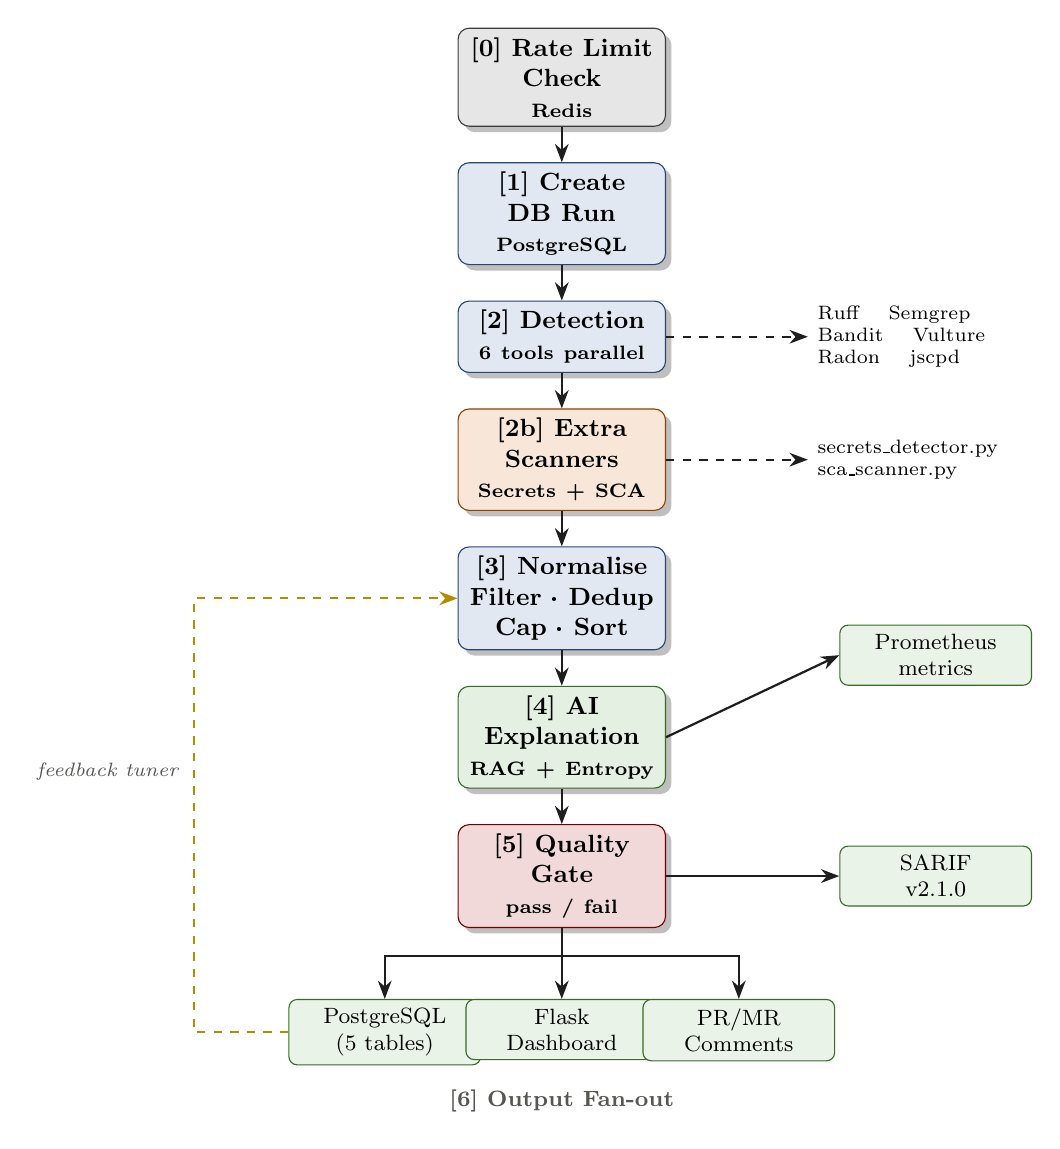
\begin{tikzpicture}[node distance=0.45cm and 1.5cm]

% ── Stage nodes (left column, top to bottom) ─────────────────────────────
\node[pipenode=stagegray] (rl) {[0] Rate Limit\\Check\\{\scriptsize Redis}};
\node[pipenode=stageblue, below=of rl] (db) {[1] Create\\DB Run\\{\scriptsize PostgreSQL}};
\node[pipenode=stageblue, below=of db] (det) {[2] Detection\\{\scriptsize 6 tools parallel}};
\node[pipenode=stageorange, below=of det] (ext) {[2b] Extra\\Scanners\\{\scriptsize Secrets + SCA}};
\node[pipenode=stageblue, below=of ext] (norm) {[3] Normalise\\Filter · Dedup\\Cap · Sort};
\node[pipenode=stagegreen, below=of norm] (ai) {[4] AI\\Explanation\\{\scriptsize RAG + Entropy}};
\node[pipenode=stagered, below=of ai] (qg) {[5] Quality\\Gate\\{\scriptsize pass / fail}};

% ── Main arrows ───────────────────────────────────────────────────────────
\foreach \a/\b in {rl/db, db/det, det/ext, ext/norm, norm/ai, ai/qg}
  \draw[pipearrow] (\a) -- (\b);

% ── Tool labels beside [2] ────────────────────────────────────────────────
\node[right=1.8cm of det, align=left, font=\scriptsize] (tools)
  {Ruff \quad Semgrep\\Bandit \quad Vulture\\Radon \quad jscpd};
\draw[pipearrow, dashed] (det.east) -- (tools.west);

% ── Extra scanner labels ──────────────────────────────────────────────────
\node[right=1.8cm of ext, align=left, font=\scriptsize] (extlbl)
  {secrets\_detector.py\\sca\_scanner.py};
\draw[pipearrow, dashed] (ext.east) -- (extlbl.west);

% ── Output fan-out from quality gate ─────────────────────────────────────
\node[fanout, below left=0.9cm and -0.3cm of qg] (pg)  {PostgreSQL\\(5 tables)};
\node[fanout, below=0.9cm of qg]                 (dash){Flask\\Dashboard};
\node[fanout, below right=0.9cm and -0.3cm of qg](pr)  {PR/MR\\Comments};
\node[fanout, right=2.2cm of qg]                 (sarif){SARIF\\v2.1.0};
\node[fanout, above right=0.0cm and 2.2cm of ai] (prom){Prometheus\\metrics};

\draw[pipearrow] (qg.south) -- ++(0,-0.35) -| (pg.north);
\draw[pipearrow] (qg.south) -- (dash.north);
\draw[pipearrow] (qg.south) -- ++(0,-0.35) -| (pr.north);
\draw[pipearrow] (qg.east)  -- (sarif.west);
\draw[pipearrow] (ai.east)  -- (prom.west);

% ── Feedback loop ─────────────────────────────────────────────────────────
\draw[pipearrow, dashed, color=ksiugold, thick]
  (pg.west) -- ++(-1.2,0) |- node[erlabel,pos=0.3,left=2pt]{feedback tuner} (norm.west);

% ── [6] output label ─────────────────────────────────────────────────────
\node[below=0.25cm of dash, font=\footnotesize\bfseries\color{stagegray}]
  {[6] Output Fan-out};

\end{tikzpicture}
\caption{ACR-QA v2.8 analysis pipeline (corrected from v2.5 architecture document).
Blue = core pipeline; orange = added in v2.8; red = quality gate; green = output.
Dashed gold arrow = feedback loop from stored findings back to normalisation
(severity override tuning via \texttt{feedback\_tuner.py}).}
\label{fig:pipeline}
\end{figure}

% ── Appendix B: ER Diagram ───────────────────────────────────────────────────
\section{Entity-Relationship Diagram}
\label{app:er}

\begin{figure}[ht]
\centering
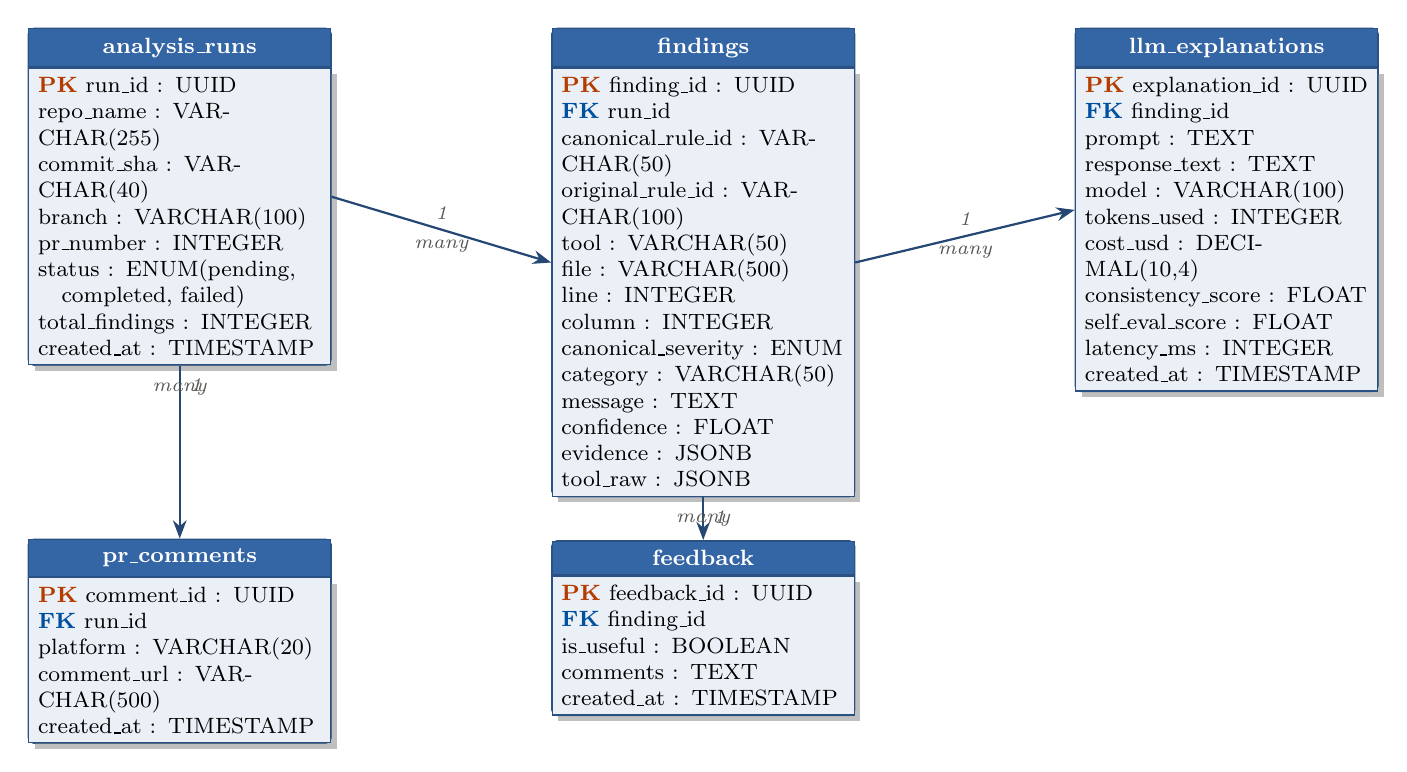
\begin{tikzpicture}[node distance=1.0cm and 2.8cm]

%% ── analysis_runs ────────────────────────────────────────────────────────
\node[erhead] (arh) {analysis\_runs};
\node[erbox, below=0pt of arh] (arb) {%
  \textcolor{pkcolor}{\textbf{PK}} run\_id : UUID\\
  repo\_name : VARCHAR(255)\\
  commit\_sha : VARCHAR(40)\\
  branch : VARCHAR(100)\\
  pr\_number : INTEGER\\
  status : ENUM(pending,\\
  \quad completed, failed)\\
  total\_findings : INTEGER\\
  created\_at : TIMESTAMP};
\begin{scope}[on background layer]
\node[draw=tableheader!80!black,fill=tableheader!5,
      fit=(arh)(arb),inner sep=0pt,rounded corners=2pt] (ar) {};
\end{scope}

%% ── findings ─────────────────────────────────────────────────────────────
\node[erhead, right=of arh] (fh) {findings};
\node[erbox, below=0pt of fh] (fb) {%
  \textcolor{pkcolor}{\textbf{PK}} finding\_id : UUID\\
  \textcolor{fkcolor}{\textbf{FK}} run\_id\\
  canonical\_rule\_id : VARCHAR(50)\\
  original\_rule\_id : VARCHAR(100)\\
  tool : VARCHAR(50)\\
  file : VARCHAR(500)\\
  line : INTEGER\\
  column : INTEGER\\
  canonical\_severity : ENUM\\
  category : VARCHAR(50)\\
  message : TEXT\\
  confidence : FLOAT\\
  evidence : JSONB\\
  tool\_raw : JSONB};
\begin{scope}[on background layer]
\node[draw=tableheader!80!black,fill=tableheader!5,
      fit=(fh)(fb),inner sep=0pt,rounded corners=2pt] (fi) {};
\end{scope}

%% ── llm_explanations ─────────────────────────────────────────────────────
\node[erhead, right=of fh] (lh) {llm\_explanations};
\node[erbox, below=0pt of lh] (lb) {%
  \textcolor{pkcolor}{\textbf{PK}} explanation\_id : UUID\\
  \textcolor{fkcolor}{\textbf{FK}} finding\_id\\
  prompt : TEXT\\
  response\_text : TEXT\\
  model : VARCHAR(100)\\
  tokens\_used : INTEGER\\
  cost\_usd : DECIMAL(10,4)\\
  consistency\_score : FLOAT\\
  self\_eval\_score : FLOAT\\
  latency\_ms : INTEGER\\
  created\_at : TIMESTAMP};
\begin{scope}[on background layer]
\node[draw=tableheader!80!black,fill=tableheader!5,
      fit=(lh)(lb),inner sep=0pt,rounded corners=2pt] (lx) {};
\end{scope}

%% ── pr_comments ──────────────────────────────────────────────────────────
\node[erhead, below=2.2cm of ar] (ph) {pr\_comments};
\node[erbox, below=0pt of ph] (pb) {%
  \textcolor{pkcolor}{\textbf{PK}} comment\_id : UUID\\
  \textcolor{fkcolor}{\textbf{FK}} run\_id\\
  platform : VARCHAR(20)\\
  comment\_url : VARCHAR(500)\\
  created\_at : TIMESTAMP};
\begin{scope}[on background layer]
\node[draw=tableheader!80!black,fill=tableheader!5,
      fit=(ph)(pb),inner sep=0pt,rounded corners=2pt] (pc) {};
\end{scope}

%% ── feedback ─────────────────────────────────────────────────────────────
\node[erhead, right=of ph] (fbkh) {feedback};
\node[erbox, below=0pt of fbkh] (fbkb) {%
  \textcolor{pkcolor}{\textbf{PK}} feedback\_id : UUID\\
  \textcolor{fkcolor}{\textbf{FK}} finding\_id\\
  is\_useful : BOOLEAN\\
  comments : TEXT\\
  created\_at : TIMESTAMP};
\begin{scope}[on background layer]
\node[draw=tableheader!80!black,fill=tableheader!5,
      fit=(fbkh)(fbkb),inner sep=0pt,rounded corners=2pt] (fbk) {};
\end{scope}

%% ── Relationships ────────────────────────────────────────────────────────
% analysis_runs 1 ──< findings
\draw[errel] (ar.east) -- node[erlabel,above]{1} node[erlabel,below]{many} (fi.west);
% findings 1 ──< llm_explanations
\draw[errel] (fi.east) -- node[erlabel,above]{1} node[erlabel,below]{many} (lx.west);
% analysis_runs 1 ──< pr_comments
\draw[errel] (ar.south) -- node[erlabel,right]{1} ++(0,-0.5) -|
             node[erlabel,above]{many} (pc.north);
% findings 1 ──< feedback
\draw[errel] (fi.south) -- node[erlabel,right]{1} ++(0,-0.5) -|
             node[erlabel,above]{many} (fbk.north);

\end{tikzpicture}
\caption{ACR-QA provenance database ER diagram.
\textcolor{pkcolor}{\textbf{PK}} = primary key;
\textcolor{fkcolor}{\textbf{FK}} = foreign key (CASCADE on delete).
All relationships are one-to-many.
The \texttt{llm\_explanations} table stores full prompt/response provenance
for hallucination auditing and cost tracking.}
\label{fig:er}
\end{figure}

% ── Appendix C: Database DDL ─────────────────────────────────────────────────
\section{Database Schema SQL (DDL)}
\label{app:ddl}

\begin{lstlisting}[language=SQL,caption={ACR-QA PostgreSQL schema v2.8 --- full DDL}]
CREATE TABLE analysis_runs (
    run_id         UUID PRIMARY KEY DEFAULT gen_random_uuid(),
    repo_name      VARCHAR(255) NOT NULL,
    commit_sha     VARCHAR(40),
    branch         VARCHAR(100),
    pr_number      INTEGER,
    status         VARCHAR(20) NOT NULL
                   CHECK (status IN ('pending','completed','failed')),
    total_findings INTEGER DEFAULT 0,
    created_at     TIMESTAMP NOT NULL DEFAULT NOW()
);

CREATE TABLE findings (
    finding_id         UUID PRIMARY KEY DEFAULT gen_random_uuid(),
    run_id             UUID NOT NULL
                       REFERENCES analysis_runs(run_id) ON DELETE CASCADE,
    canonical_rule_id  VARCHAR(50) NOT NULL,
    original_rule_id   VARCHAR(100),
    tool               VARCHAR(50) NOT NULL,
    file               VARCHAR(500) NOT NULL,
    line               INTEGER NOT NULL,
    column             INTEGER,
    end_line           INTEGER,
    canonical_severity VARCHAR(10) NOT NULL
                       CHECK (canonical_severity IN ('high','medium','low')),
    category           VARCHAR(50),
    message            TEXT NOT NULL,
    description        TEXT,
    confidence         FLOAT,
    evidence           JSONB,
    tool_raw           JSONB NOT NULL,
    UNIQUE(run_id, canonical_rule_id, file, line)
);

CREATE TABLE llm_explanations (
    explanation_id   UUID PRIMARY KEY DEFAULT gen_random_uuid(),
    finding_id       UUID NOT NULL
                     REFERENCES findings(finding_id) ON DELETE CASCADE,
    prompt           TEXT NOT NULL,
    response_text    TEXT NOT NULL,
    model            VARCHAR(100) NOT NULL,
    tokens_used      INTEGER,
    cost_usd         DECIMAL(10,4),
    consistency_score FLOAT,
    self_eval_score  FLOAT,
    latency_ms       INTEGER,
    status           VARCHAR(20) DEFAULT 'success',
    created_at       TIMESTAMP NOT NULL DEFAULT NOW()
);

CREATE TABLE pr_comments (
    comment_id  UUID PRIMARY KEY DEFAULT gen_random_uuid(),
    run_id      UUID NOT NULL
                REFERENCES analysis_runs(run_id) ON DELETE CASCADE,
    platform    VARCHAR(20) CHECK (platform IN ('github','gitlab')),
    comment_url VARCHAR(500),
    created_at  TIMESTAMP NOT NULL DEFAULT NOW()
);

CREATE TABLE feedback (
    feedback_id UUID PRIMARY KEY DEFAULT gen_random_uuid(),
    finding_id  UUID NOT NULL
                REFERENCES findings(finding_id) ON DELETE CASCADE,
    is_useful   BOOLEAN NOT NULL,
    comments    TEXT,
    created_at  TIMESTAMP NOT NULL DEFAULT NOW()
);

-- Performance indexes
CREATE INDEX idx_findings_run_sev  ON findings(run_id, canonical_severity);
CREATE INDEX idx_findings_category ON findings(category);
CREATE INDEX idx_llm_cost          ON llm_explanations(created_at, cost_usd);
CREATE INDEX idx_feedback_finding  ON feedback(finding_id);
\end{lstlisting}

% ── Appendix D: Canonical Finding JSON ───────────────────────────────────────
\section{Sample Canonical Finding (JSON)}
\label{app:json}

\begin{lstlisting}[language=Python,caption={Canonical finding --- SQL injection (DVPWA)}]
{
  "finding_id":        "f7a3c2e1-4b5d-6e7f-8a9b-0c1d2e3f4a5b",
  "canonical_rule_id": "SECURITY-027",
  "original_rule_id":  "B608",
  "tool":              "bandit",
  "file":              "sqli/dao/student.py",
  "line":              42,
  "canonical_severity":"high",
  "category":          "security",
  "message":           "Possible SQL injection via string formatting",
  "confidence":        0.92,
  "evidence": {
    "snippet":        "query = \"SELECT * FROM students WHERE id = '%s'\" % uid",
    "context_before": ["def get_student(uid):", "    cur = db.cursor()"],
    "context_after":  ["    return cur.fetchall()"]
  },
  "tool_raw": {
    "tool_name":          "bandit",
    "original_severity":  "MEDIUM",
    "original_confidence":"MEDIUM"
  }
}
\end{lstlisting}

% ── Appendix E: .acrqa.yml Template ─────────────────────────────────────────
\section{Documented \texttt{.acrqa.yml} Policy Template}
\label{app:yml}

\begin{lstlisting}[language=Python,caption={.acrqa.yml --- annotated v2.8 template}]
# ACR-QA Policy Configuration
# Version-control this file alongside your code.

rules:
  disabled_rules:
    - IMPORT-001       # wildcard imports are intentional here
  severity_overrides:
    VAR-001: high      # unused variables unacceptable in this project

analysis:
  ignore_paths:
    - __pycache__
    - .venv
    - node_modules
    - "migrations/*"

reporting:
  min_severity: medium  # suppress low-severity noise in CI output

quality_gate:
  max_high:     0       # zero tolerance for high-severity findings
  max_medium:  20       # calibrated from 9-repo study (was: 10)
  max_total:  200       # hard cap on total findings
  max_security: 3       # allow a few low-risk security findings

autofix:
  enabled: true
  auto_apply_confidence: 80  # only auto-apply fixes >= 80% confidence

ai:
  enabled: true
  max_explanations: 50       # cap API calls per run (cost control)
  model: llama-3.1-8b-instant
\end{lstlisting}

% ── Appendix F: OWASP Coverage ───────────────────────────────────────────────
\section{OWASP Top 10 (2021) Coverage}
\label{app:owasp}

\begin{table}[ht]
\centering
\caption{ACR-QA v2.8 OWASP Top 10 Coverage}
\begin{tabular}{llcp{5.5cm}}
\toprule
\textbf{Category} & \textbf{Status} & \textbf{Rules} & \textbf{CWEs}\\
\midrule
A01 Broken Access Control    & \checkmark & 2  & CWE-200, CWE-284, CWE-352\\
A02 Cryptographic Failures   & \checkmark & 7  & CWE-259, CWE-327, CWE-328\\
A03 Injection                & \checkmark & 4  & CWE-79, CWE-89, CWE-78\\
A04 Insecure Design          & \checkmark & 3  & CWE-209, CWE-256\\
A05 Security Misconfiguration& \checkmark & 6  & CWE-16, CWE-611\\
A06 Vulnerable Components    & \checkmark & 6  & CWE-1104\\
A07 Auth Failures            & \checkmark & 3  & CWE-287, CWE-384\\
A08 Data Integrity           & \checkmark & 2  & CWE-502\\
A09 Logging Failures         & Planned    & 0  & CWE-778 (runtime analysis needed)\\
A10 SSRF                     & \checkmark & 2  & CWE-918\\
\bottomrule
\multicolumn{4}{l}{\small 9/10 categories covered. A09 requires dynamic log
analysis; planned for v3.0.}\\
\end{tabular}
\end{table}

% ── Appendix G: User Study Materials ─────────────────────────────────────────
\section{User Study Design Summary}
\label{app:user}

\textbf{Objective:} measure the impact of ACR-QA AI-powered explanations on
developer understanding and fix speed versus raw tool output.

\textbf{Design:} between-subjects A/B comparison, 5 participants.  Group A
(control) sees raw Bandit output.  Group B (treatment) sees ACR-QA output with
AI explanations, severity labels, and code fix examples.

\textbf{Metrics collected per finding:} understanding rating (1--5), fix
confidence (1--5), time to write a fix (seconds), correct fix (yes/no).

\textbf{Statistical tests:} Mann-Whitney U (non-parametric; $n$\,=\,5 per group);
Fisher's exact test for correct-fix proportion; Cohen's $d$ for effect size.

\textbf{Status:} materials generated; participant recruitment in progress;
data collection planned before June 2026 final report submission.

\end{document}
